\chapter{Evaluation}

\section{Introduction}
This chapter will...

\section{Evaluation Metrics for Classification}
The following four metrics were used to evaluate the classifiers:
\begin{enumerate}
    \item Precision
    \item Recall
    \item Accuracy
    \item F1-Score
\end{enumerate}

\subsection*{Precision}
Precision is a measure of the classifiers 'exactness'. It is the percentage of everything classified as a 'review', 'some content', or 'irrelevant' that was classified correctly. Precision is the total number of true positives divided by the total number of positives (true positives and false positives).
\begin{center}
    $Precision\ =\ \cfrac{True\ Positives}{True\ Positives\ +\ False\ Positives}$
\end{center}
A low precision value can indicate a large number of false positives i.e. a large number of tweets incorrectly classified as as a 'review', 'some content', or 'irrelevant'. A high precision value indicates that the majority of what was classified, was classified correctly. You could however, have a very high precision in the case where only a small potion of samples were actually classified but of these the majority were classified correctly.

\subsection*{Recall}
Recall is a measure of the classifiers 'completeness'. It is the percentage of everything that should have been classified as a 'review', 'some content', or 'irrelevant' that was classified correctly. Recall is the total number of true positives divided by the total number of true positives and false negatives.
\begin{center}
    $Recall\ =\ \cfrac{True\ Positives}{True\ Positives\ +\ False\ Negatives}$
\end{center}
A low recall value can indicate there are a large number of false negatives, predictions that should hve been classified but were not. A high recall value indicates that the majority of tweets that should have been classified as a 'review', 'some content', or 'irrelevant' that was classified correctly.

\subsection*{Accuracy}
Accuracy is the total number of samples predicted correctly. It is the percentage of the tweets that were classified correctly. Accuracy is the total number of correct predictions (true positives and true negatives) over the total number of predictions. 
\begin{center}
    $Accuracy\ =\ \cfrac{True\ Positives\ +\ True Negatives}{Total Predictions}$
\end{center}
The higher the accuracy score the better, but a high accuracy does not always give an accurate representation of the situation. It will not identify a class imbalance.

\subsection*{F1-Score}
F1-Score is the harmonic mean of precision and recall. It is also called the F-Score or F-Measure. The F1-Score shows the balance between precision and recall. 
\begin{center}
    $F1-Score\ =\ \cfrac{2 \times\ Precision\ \times\ Recall}{Precision\ +\ Recall}$
\end{center}
The higher the F1-Score the better.

\section{Evaluation Metrics for Recommender Systems}

\section{Results and Analysis}

\section{Discussion of Results}

\section{Summary}

\subsection*{Limitations}

\begin{figure}[h!]
\centering
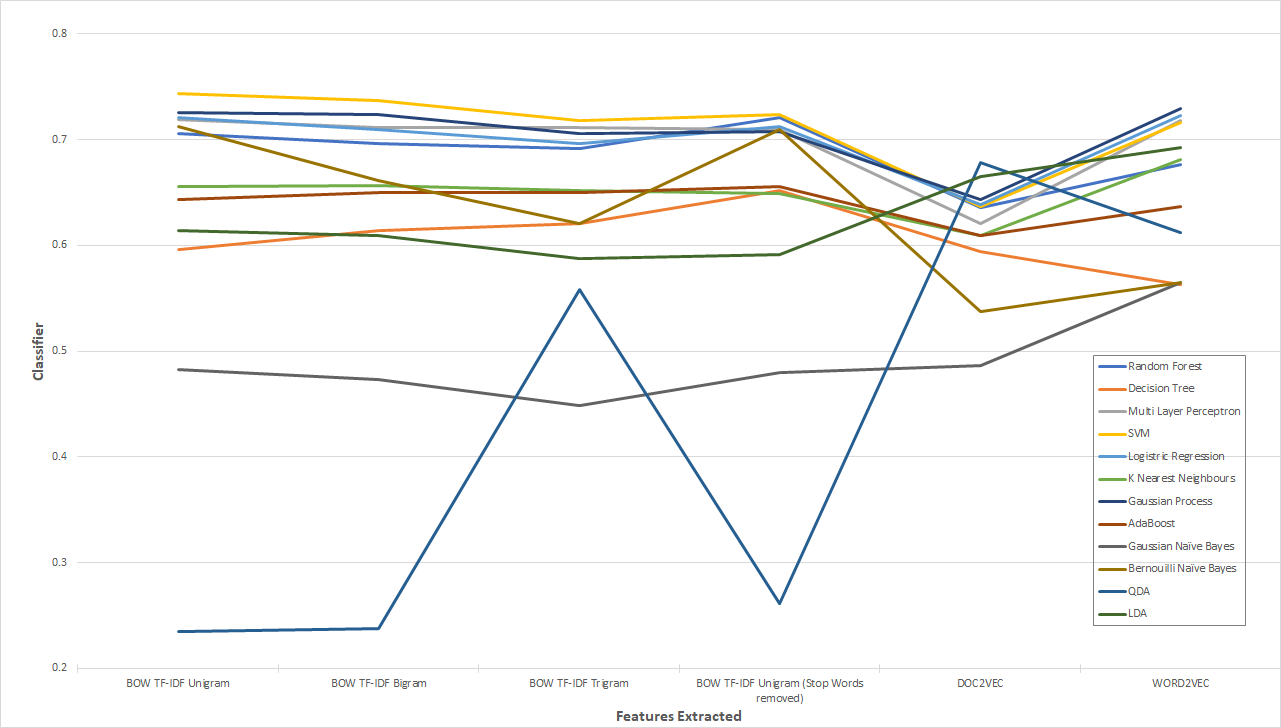
\includegraphics[width=1\textwidth]{evaluation/accuracy_graph.png}
\caption{\label{fig:accuracy} Accuracy Graph}
\end{figure}

\begin{figure}[h!]
\centering
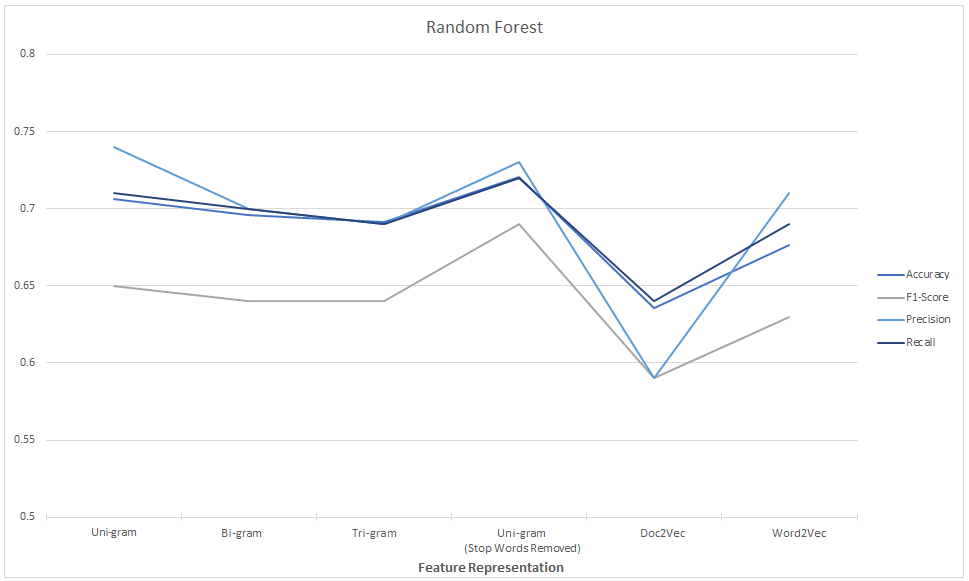
\includegraphics[width=1\textwidth]{evaluation/random_forest_graph.png}
\caption{\label{graph:randomforest} Random Forest Graph}
\end{figure}

% *** ACCURACY ***
\begin{table}[]
\setlength\extrarowheight{5pt}
\resizebox{\textwidth}{!}{
\begin{tabular}{ccccccc}
\specialrule{1.5pt}{1pt}{1pt}
 & \textbf{Uni-gram} & \textbf{Bi-gram} & \textbf{Tri-gram} & \textbf{\begin{tabular}[c]{@{}c@{}}Uni-gram \\ (No Stop Words)\end{tabular}} & \textbf{Doc2Vec} & \textbf{Word2Vec} \\ \specialrule{1.5pt}{1pt}{1pt}
\textbf{RF} & 0.706 & 0.696 & 0.691 & 0.721 & 0.635 & 0.677 \\ \hline
\rowcolor[HTML]{EFEFEF} 
\textbf{DT} & 0.596 & 0.614 & 0.621 & 0.652 & 0.594 & 0.563 \\ \hline
\textbf{MLP} & 0.719 & 0.711 & 0.711 & 0.709 & 0.621 & 0.718 \\ \hline
\rowcolor[HTML]{EFEFEF} 
\textbf{SVM} & 0.744 & 0.737 & 0.718 & 0.724 & 0.637 & 0.716 \\ \hline
\textbf{LR} & 0.721 & 0.709 & 0.696 & 0.713 & 0.639 & 0.722 \\ \hline
\rowcolor[HTML]{EFEFEF} 
\textbf{KNN} & 0.655 & 0.657 & 0.652 & 0.649 & 0.609 & 0.681 \\ \hline
\textbf{GP} & 0.726 & 0.724 & 0.706 & 0.708 & 0.644 & 0.729 \\ \hline
\rowcolor[HTML]{EFEFEF} 
\textbf{AB} & 0.644 & 0.650 & 0.650 & 0.655 & 0.609 & 0.637 \\ \hline
\textbf{GNB} & 0.483 & 0.473 & 0.448 & 0.479 & 0.486 & 0.565 \\ \hline
\rowcolor[HTML]{EFEFEF} 
\textbf{BNB} & 0.713 & 0.662 & 0.621 & 0.709 & 0.537 & 0.565 \\ \hline
\textbf{QDA} & 0.235 & 0.238 & 0.558 & 0.261 & 0.678 & 0.612 \\ \hline
\rowcolor[HTML]{EFEFEF} 
\textbf{LDA} & 0.614 & 0.609 & 0.588 & 0.591 & 0.665 & 0.693 \\ \hline
\end{tabular}}
\caption{Accuracy of Classifiers for different Feature Representations}
\label{Table:accuracy}
\end{table}

% *** F1 SCORE ***
\begin{table}[]
\setlength\extrarowheight{5pt}
\resizebox{\textwidth}{!}{
\begin{tabular}{ccccccc}
\specialrule{1.5pt}{1pt}{1pt}
 & \textbf{Uni-gram} & \textbf{Bi-gram} & \textbf{Tri-gram} & \textbf{\begin{tabular}[c]{@{}c@{}}Uni-gram \\ (No Stop Words)\end{tabular}} & \textbf{Doc2Vec} & \textbf{Word2Vec} \\ \specialrule{1.5pt}{1pt}{1pt}
\textbf{RF} & 0.65 & 0.64 & 0.64 & 0.69 & 0.59 & 0.63 \\ \hline
\rowcolor[HTML]{EFEFEF} 
\textbf{DT} & 0.59 & 0.58 & 0.6 & 0.63 & 0.56 & 0.54 \\ \hline
\textbf{MLP} & 0.7 & 0.69 & 0.69 & 0.69 & 0.57 & 0.71 \\ \hline
\rowcolor[HTML]{EFEFEF} 
\textbf{SVM} & 0.73 & 0.73 & 0.71 & 0.71 & 0.63 & 0.71 \\ \hline
\textbf{LR} & 0.7 & 0.69 & 0.68 & 0.69 & 0.6 & 0.71 \\ \hline
\rowcolor[HTML]{EFEFEF} 
\textbf{KNN} & 0.62 & 0.62 & 0.62 & 0.61 & 0.55 & 0.67 \\ \hline
\textbf{GP} & 0.71 & 0.72 & 0.7 & 0.7 & 0.61 & 0.72 \\ \hline
\rowcolor[HTML]{EFEFEF} 
\textbf{AB} & 0.62 & 0.63 & 0.62 & 0.63 & 0.59 & 0.63 \\ \hline
\textbf{GNB} & 0.51 & 0.49 & 0.47 & 0.5 & 0.51 & 0.58 \\ \hline
\rowcolor[HTML]{EFEFEF} 
\textbf{BNB} & 0.72 & 0.67 & 0.64 & 0.71 & 0.55 & 0.58 \\ \hline
\textbf{QDA} & 0.19 & 0.19 & 0.48 & 0.23 & 0.61 & 0.55 \\ \hline
\rowcolor[HTML]{EFEFEF} 
\textbf{LDA} & 0.62 & 0.62 & 0.6 & 0.6 & 0.66 & 0.69 \\ \hline
\end{tabular}}
\caption{F1-Score of Classifiers for different Feature Representations}
\label{Table:f1score}
\end{table}

% *** PRECISION ***
\begin{table}[]
\setlength\extrarowheight{5pt}
\resizebox{\textwidth}{!}{
\begin{tabular}{ccccccc}
\specialrule{1.5pt}{1pt}{1pt}
 & \textbf{Uni-gram} & \textbf{Bi-gram} & \textbf{Tri-gram} & \textbf{\begin{tabular}[c]{@{}c@{}}Uni-gram \\ (No Stop Words)\end{tabular}} & \textbf{Doc2Vec} & \textbf{Word2Vec} \\ \specialrule{1.5pt}{1pt}{1pt}
\textbf{RF} & 0.74 & 0.7 & 0.69 & 0.73 & 0.59 & 0.71 \\ \hline
\rowcolor[HTML]{EFEFEF} 
\textbf{DT} & 0.58 & 0.58 & 0.59 & 0.63 & 0.56 & 0.54 \\ \hline
\textbf{MLP} & 0.71 & 0.7 & 0.7 & 0.7 & 0.59 & 0.71 \\ \hline
\rowcolor[HTML]{EFEFEF} 
\textbf{SVM} & 0.74 & 0.73 & 0.71 & 0.71 & 0.62 & 0.71 \\ \hline
\textbf{LR} & 0.72 & 0.7 & 0.68 & 0.7 & 0.61 & 0.71 \\ \hline
\rowcolor[HTML]{EFEFEF} 
\textbf{KNN} & 0.62 & 0.62 & 0.62 & 0.61 & 0.54 & 0.67 \\ \hline
\textbf{GP} & 0.72 & 0.71 & 0.69 & 0.7 & 0.61 & 0.72 \\ \hline
\rowcolor[HTML]{EFEFEF} 
\textbf{AB} & 0.62 & 0.63 & 0.62 & 0.64 & 0.57 & 0.63 \\ \hline
\textbf{GNB} & 0.6 & 0.63 & 0.63 & 0.59 & 0.59 & 0.64 \\ \hline
\rowcolor[HTML]{EFEFEF} 
\textbf{BNB} & 0.73 & 0.71 & 0.71 & 0.72 & 0.58 & 0.65 \\ \hline
\textbf{QDA} & 0.76 & 0.73 & 0.67 & 0.79 & 0.57 & 0.59 \\ \hline
\rowcolor[HTML]{EFEFEF} 
\textbf{LDA} & 0.64 & 0.65 & 0.63 & 0.62 & 0.66 & 0.69 \\ \hline
\end{tabular}}
\caption{Precision of Classifiers for different Feature Representations}
\label{Table:precision}
\end{table}

% *** RECALL ***
\begin{table}[]
\setlength\extrarowheight{5pt}
\resizebox{\textwidth}{!}{
\begin{tabular}{ccccccc}
\specialrule{1.5pt}{1pt}{1pt}
 & \textbf{Uni-gram} & \textbf{Bi-gram} & \textbf{Tri-gram} & \textbf{\begin{tabular}[c]{@{}c@{}}Uni-gram \\ (No Stop Words)\end{tabular}} & \textbf{Doc2Vec} & \textbf{Word2Vec} \\ \specialrule{1.5pt}{1pt}{1pt}
\textbf{RF} & 0.71 & 0.7 & 0.69 & 0.72 & 0.64 & 0.69 \\ \hline
\rowcolor[HTML]{EFEFEF} 
\textbf{DT} & 0.6 & 0.61 & 0.62 & 0.65 & 0.59 & 0.56 \\ \hline
\textbf{MLP} & 0.72 & 0.71 & 0.71 & 0.71 & 0.62 & 0.72 \\ \hline
\rowcolor[HTML]{EFEFEF} 
\textbf{SVM} & 0.74 & 0.74 & 0.72 & 0.72 & 0.64 & 0.72 \\ \hline
\textbf{LR} & 0.72 & 0.71 & 0.7 & 0.71 & 0.64 & 0.72 \\ \hline
\rowcolor[HTML]{EFEFEF} 
\textbf{KNN} & 0.66 & 0.66 & 0.65 & 0.65 & 0.61 & 0.68 \\ \hline
\textbf{GP} & 0.73 & 0.72 & 0.71 & 0.71 & 0.64 & 0.73 \\ \hline
\rowcolor[HTML]{EFEFEF} 
\textbf{AB} & 0.64 & 0.65 & 0.65 & 0.66 & 0.61 & 0.64 \\ \hline
\textbf{GNB} & 0.48 & 0.47 & 0.45 & 0.48 & 0.49 & 0.56 \\ \hline
\rowcolor[HTML]{EFEFEF} 
\textbf{BNB} & 0.71 & 0.66 & 0.62 & 0.71 & 0.54 & 0.56 \\ \hline
\textbf{QDA} & 0.23 & 0.24 & 0.56 & 0.26 & 0.68 & 0.61 \\ \hline
\rowcolor[HTML]{EFEFEF} 
\textbf{LDA} & 0.61 & 0.61 & 0.59 & 0.59 & 0.67 & 0.69 \\ \hline
\end{tabular}}
\caption{Recall of Classifiers for different Feature Representations}
\label{Table:recall}
\end{table}


